\section{Техніко-економічне обґрунтування проекту}
Мета даного розділу --- провести розрахунок сукупної величини витрат, пов'язаних з розробкою програмної компоненти для аналізу стійкості функціонування логістичних систем.

Витрати на розробку будуть проводитись за наступними пунктами:
\begin{itemize}
	\item витрат на апаратне забезпечення;
	\item витрат на програмне забезпечення;
	\item витрат на зовнішні постачальники послуг;
	\item витрат на оплату праці.
\end{itemize}

Для розробки програмних компонентів агентної платформи використовується мова програмування Kotlin.
Проект потребує спеціалістів які володіють зазначеною мовою на рівні не нижче середнього на ринку, через високу складність конструювання програмного забезпечення.
Даний проект розробляється командою з трьох програмних інженерів зазначеної спеціалізації, проектного менеджера, експерта з логістичних систем та тестувальника.
Термін розробки складає два року.

В якості методології розробки буде використана методологія XP.

\subsection{Апаратне забезпечення}
Для команди розробників необхідні апаратні компоненти які задовольняють таким вимогам:
\begin{itemize}
	\item процесор: Intel core i7 5 покоління;
	\item оперативна пам'ять: DDR4 16 GB;
	\item внутрішня пам'ять: SSD 256 GB.
\end{itemize}

Оптимальною конфігурацією для роботи буде ноутбук MacBook Pro 2015 року з 16 ГБ оперативної пам'яті.

Для проектного менеджера необхідні апаратні компоненти які задовольняють таким вимогам:
\begin{itemize}
	\item процесор: Intel core i3 5 покоління;
	\item оперативна пам'ять: DDR4 4 ГБ;
	\item внутрішня пам'ять: SSD 256 ГБ.
\end{itemize}

Оптимальною конфігурацією для роботи буде ноутбук MacBook Air 2015 року з 4 ГБ оперативної пам'яті.

Для експерта з логістичних систем та тестувальника необхідні апаратні компоненти які задовольняють таким вимогам:
\begin{itemize}
	\item процесор: Intel core i7 5 покоління;
	\item оперативна пам'ять: DDR4 8 ГБ;
	\item внутрішня пам'ять: SSD 256 ГБ.
\end{itemize}

Оптимальною конфігурацією для роботи буде ноутбук MacBook 2015 року з 8 ГБ оперативної пам'яті.

Вартість кожної апаратної компоненти представлена в таблиці~\ref{tab:economy_hardware}.

{
\tabulinesep=1.2mm
\begin{longtabu} to \textwidth {|X[3,l]|X[1,c]|}
	\caption{Вартість апаратних компонентів необхідних для команди}
	\label{tab:economy_hardware} \\
	\hline
	Модель ноутбука & Вартість, грн. \\
	\hline
	\endfirsthead
	\caption*{Закінчення таблиці \thetable{}}\\
	\hline
	Модель ноутбука & Вартість, грн. \\
	\hline
	\endhead

	MacBook Pro 15 2015 Retina Z0W60002T & $35499$~\cite{MacBookProPrice} \\ \hline
	MacBook Pro 15 2015 Retina Z0W70001U & $43299$~\cite{MacBookProPrice} \\ \hline
	MacBook Air 2015 Z0X5000BR & $29999$~\cite{MacBookAirPrice} \\ \hline
\end{longtabu}
}

Вартість апаратного забезпечення для команди розробників:
\[
	C_{hw:dev} = 43299 \cdot 3 = 129897 \textup{ грн.}
\]
, для проектного менеджера:
\[
	C_{hw:pm} = 29999 = 29999 \textup{ грн.}
\]
, для експерта з логістичних систем:
\[
	C_{hw:expert} = 35499 = 35499 \textup{ грн.}
\]
, для тестувальника:
\[
	C_{hw:test} = 35499 = 35499 \textup{ грн.}
\]

Загальна вартість апаратних компонентів необхідних для проектної команди дорівнює:
\begin{gather*}
	C_{hw} = C_{hw:dev} + C_{hw:pm} + C_{hw:expert} + C_{hw:dev} = \\
	= 129897 + 29999 + 35499 + 35499 = \\
	= 230894 \textup{ грн.}
\end{gather*}

\subsection{Витрати на оплату праці}
Вартість роботи проектної команди зображена в таблицях~\ref{tab:economy_hr_1},~\ref{tab:economy_hr_2}.

	{
		\tabulinesep=1.2mm
		\begin{longtabu} to \textwidth {|X[4,l]|X[1,l]|X[3,l]|}
			\caption{Розподіл заробітної плати проектної команди}
			\label{tab:economy_hr_1} \\
			\hline
			Учасник проекту & Посада & Заробітна плата, дол. / год. \\
			\hline
			\endfirsthead
			\caption*{Закінчення таблиці \thetable{}}\\
			\hline
			Учасник проекту & Посада & Заробітна плата, дол. / год. \\
			\hline
			\endhead

			Менеджер проекту & Middle & $8.25$~\cite{SalaryProgrammer} \\ \hline
			Kotlin розробник №1 & Senior & $15.5$~\cite{SalaryProgrammer} \\ \hline
			Kotlin розробник №2 & Middle & $9$~\cite{SalaryProgrammer} \\ \hline
			Kotlin розробник №3 & Middle & $9$~\cite{SalaryProgrammer} \\ \hline
			Експерт в логістичних системах & Middle & $11$~\cite{SalaryLogisticExpert} \\ \hline
			QA інженер & Middle & $6$~\cite{SalaryProgrammer} \\ \hline
		\end{longtabu}
	}
	{
		\small
		\tabulinesep=1.2mm
		\begin{longtabu} to \textwidth {|X[2,l]|X[1,l]|X[1,l]|X[1,l]|X[1,l]|X[1,l]|X[1,l]|}
			\caption{Розподіл робочих годин та вартості роботи проектної команди}
			\label{tab:economy_hr_2} \\
			\hline
			Фаза проекту & Менеджер проекту, год. & Kotlin розробник №1, год. & Kotlin розробник №2, год. & Kotlin розробник №3, год. & Експерт в логістичних системах, год. & QA інженер, год. \\
			\hline
			\endfirsthead
			\caption*{Закінчення таблиці \thetable{}}\\
			\hline
			Фаза проекту & Менеджер проекту, год. & Kotlin розробник №1, год. & Kotlin розробник №2, год. & Kotlin розробник №3, год. & Експерт в логістичних системах, год. & QA інженер, год. \\
			\hline
			\endhead

			Початкова фаза (1-6 місяць) & 200 & 100 & 0 & 0 & 100 & 0 \\ \hline
			Фаза уточнення (7-9 місяць) & 200 & 200 & 50 & 50 & 200 & 50 \\ \hline
			Фаза конструювання (10-15 місяць) & 100 & 200 & 200 & 200 & 50 & 200 \\ \hline
			Фаза впровадження (10-15 місяць) & 100 & 100 & 150 & 150 & 50 & 200 \\ \hline
			$\sum$ & 600 & 600 & 400 & 400 & 400 & 450 \\ \hline
		\end{longtabu}
	}

Загальна вартість роботи проектної команди:
\begin{gather*}
	C_{hr} = \\ = 600 \cdot 8.25 + 600 \cdot 15.5 + 400 \cdot 9 + 400 \cdot 9 + 400 \cdot 11 + 450 \cdot 6 = \\ = 28550 \textup{ дол.}
\end{gather*}

Згідно із курсом долара~\cite{Dollar} (станом на 20.04.20) вартість на команду розробки у гривнях становить:
\begin{gather*}
	C_{hr} = 28550 \cdot 27.2 = 776560 \textup{ грн.}
\end{gather*}

\subsection{Витрати на програмне забезпечення}
На усіх компьютерах команди буде встановлена безкоштовна операційна система mac OS. Серед основних цілей mac os -- надання сучасного й водночас стабільного програмного забезпечення для пересічного користувача із сильним акцентом на простоту встановлення та користування~\cite{MacOS}.

Розробка програмних компонентів агентної платформи буде виконуватись із використання середовища для розробки Intellij Idea Ultimate Edition. Згідно із курсом долара~\cite{Dollar} (станом на 20.04.20) вартість на використання середовища у гривнях становить~\cite{IDEA}:
\[
	C_{sw:idea} = 449 \cdot 1.5 \cdot 3 \cdot 27.2 = 54957.6 \textup{ грн.}
\]

Для забезпечення приватності, версіонування та збереження коду, та тестування системи буде використана система контролю версій Git, а саме холдінг GitHub. Згідно із курсом долара~\cite{Dollar} (станом на 20.04.20) вартість на використання сервісу у гривнях становить~\cite{GitHubPricing}:
\[
	C_{sw:github} = 4 \cdot 18 \cdot 6 \cdot 27.2 = 11750.4 \textup{ грн.}
\]

Для моніторінга виконання задач проект буде використовуватись
система Jira. Jira --- система відстеження помилок, призначена для організації спілкування з користувачами, і для управління проектами. Згідно із курсом долара~\cite{Dollar} (станом на 20.04.20) вартість на використання сервісу у гривнях становить~\cite{JiraPricing}:
\[
	C_{sw:jira} = 14 \cdot 18 \cdot 6 \cdot 27.2 = 41126.4 \textup{ грн.}
\]

Загальна сума витрат на програмне забезпечення становить:
\begin{gather*}
	C_{sw} = C_{sw:idea} + C_{sw:github} + C_{sw:jira} = \\
	= 54957.6 + 11750.4 + 41126.4 = \\
	= 107834.4 \textup{ грн.}
\end{gather*}

\subsection{Зовнішні постачальники послуг}
Витрати на зовнішніх постачальників послуг будемо брати за півроку роботи програмної компоненти. В якості постачальників було обрано інтернет-провайдер <<Тріолан>>, вартість тарифних пакетів зображено на рисунку~\ref{fig:triolan}.

\begin{figure}[H]
	\centering
	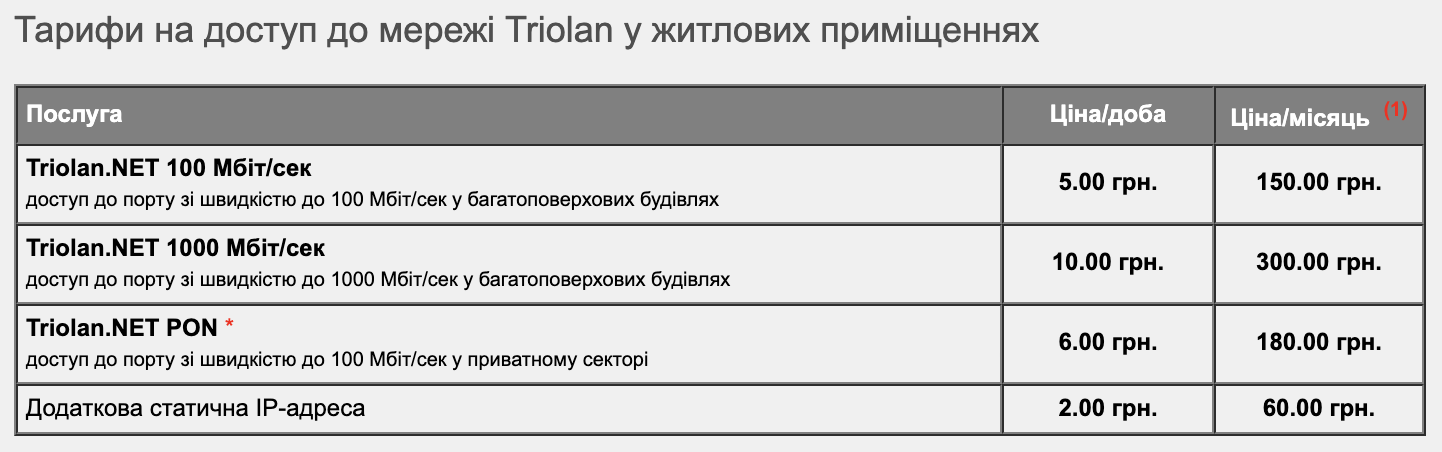
\includegraphics[width=0.8\textwidth]{triolan}
	\caption{Тарифні плани інтернет-провайдеру <<Тріолан>>~\cite{TriolanPrice}}
	\label{fig:triolan}
\end{figure} 

Витрати на інтернет доступ (рисунок~\ref{fig:triolan}):
\begin{gather*}
	C_{misc:triolan} = 150 * 6 * 18 = 16200 \textup{ грн.}
\end{gather*}

\subsection{Загальні витрати на проект}
Результати загальних розрахунків витрат на проект зведені у таблицю~\ref{tab:economy_total}.

{
	\tabulinesep=1.2mm
	\begin{longtabu} to \textwidth {|X[4,l]|X[1,l]|}
		\caption{Загальні витрати}
		\label{tab:economy_total} \\
		\hline
		Найменування витрат & Витрати \\
		\hline
		\endfirsthead
		\caption*{Закінчення таблиці \thetable{}}\\
		\hline
		Найменування витрат & Витрати \\
		\hline
		\endhead

		Апаратне забезпечення & $230894$ грн. \\ \hline
		Оплата праці & $776560$ грн. \\ \hline
		Програмне забезпечення & $107834.4$ грн. \\ \hline
		Зовнішні постачальники послуг & $16200$ грн. \\ \hline
		$\sum$ & $1131488.4$ грн. \\ \hline
	\end{longtabu}
}

В даному розділі було виконано розрахунки собівартості на розробку \acrshort{sw} для аналізу стійкості функціонування логістичних систем. В результаті було отримано, що на виконання робіт по розробці буде витрачено півтора року та повна собівартість $1131488.4$ грн. Собівартість складається з витрат на апаратне забезпечення, програмне забезпечення, заробітну плату та витрат на зовнішніх постачальників послуг.
